\documentclass[12pt]{article}

\usepackage{graphicx}
\usepackage[left=0.8in,top=0.8in,right=0.8in,bottom=0.8in]{geometry}
\usepackage{titling}
\usepackage{sectsty}
\usepackage{comment}
\usepackage{amsmath}
\usepackage{amssymb}
\usepackage{siunitx}
\usepackage{float}
\graphicspath{{img/}}
\setlength\parindent{24pt}
\sectionfont{\fontsize{12}{16}\selectfont}

\title{\vspace{-2.5em} \Large \textbf{Homework \#4}}
\author{Justin Kang \\ AST 381: Planetary Astrophysics}
\date{\vspace{-0.75em} November 16, 2017}

\begin{document}
\maketitle

% The system that we’ll be using is HD 209458.
% To simplify matters, we’re going to use a Hot Jupiter with a circular orbit, and we aren’t going to try fitting transit data or anything silly like that.
\noindent The system we are interested in is HD 209458 and its planet. For the sake of simplicity, we assume that HD 209458 b, a hot Jupiter, is on a circular orbit - this is relatively accurate as $e = 0.014$. For this project, all literature values are taken from Laughlin et al. (2005) \cite{rvdata}.\\
% You should plan to fit three parameters: orbital period, Msin(i), and a time zero point. (Note that for a circular orbit, longitude of periapse is formally undefined, so I suggest defining the time zero point to be when the planet is crossing in front of the star with zero radial velocity.)
\indent We plan to fit the planet's $M\sin(i)$, orbital period, and time zero point (when the planet crosses in front of the star such that it has zero radial velocity) using MCMC. 
% Don’t worry about multiple walkers or anything like that. Do worry about making sure you discard early steps before burn-in.
To run the MCMC, we generate a "random" first model - here 0.7 $M_\text{J}$, 3.525 days, and 2452854.8 HJD were used as they are close but not actually the real values. The initial $\chi^{2}$ value is then calculated from this for sake of comparison. Here $\chi^{2}$ compares the literature RVs with those calculated from the model. We start with the equation $$v_{*} = \frac{M_{p}}{M_{*}}v_{p} = \frac{M_{p}}{M_{*}}\left(2\pi{a}/P\right) = \frac{M_{p}}{M_{*}}\left[2\pi\left(\frac{GM_{*}P^{2}}{4\pi^{2}}\right)^{1/3}/P\right].$$ The first term we get from conservation of linear momentum in the star-planet system. Here $M_{*} = 1.14\ M_{\odot}$, and $M_{p} = M\sin(i)$ is from our model. The second term we get by applying $v = d/t$, where $d$ is the circumference of the orbit and $P$ is the orbital period from our model (as we assumed a circular orbit). The third term we get from Kepler's third law, making the approximation $M_{*} + M_{p} \approx M_{*}$. Including phase, we finally obtain the equation $$RV = v_{*}\sin\left(2\pi\frac{t_{c}-t}{P}\right),$$ where $t_{c}$ is the literature crossing time and $t$ is from our model. We then randomly perturb one parameter by sampling from a Gaussian distribution. If this perturbation lowers the $\chi^{2}$ value or passes under some probability $\alpha$ test, we accept it as a new model, updating each parameter and $\chi^{2}$. In our code we set $\alpha = \text{min}\left(1, e^{-\Delta\chi^{2}/2}\right)$ to account for both of these cases. Here the $\sigma$ in our Gaussian distributions are chosen so that we have a jump acceptance rate of $\sim20-40\%$ in each of our parameters. We then repeat this for as many iterations as we need. We also include a "burn-in" phase - here we are trying to get the MCMC to first find the extrema, so we toss out a values in the beginning. We set the number of burn-in iterations as 5000 and total iterations as 1000000, which worked well empirically.\\
% You should track the acceptance rate on proposed jumps for each parameter. Recall from our discussion in class that you don’t want a value that’s too high (or it takes a long time to mix) or too low (wasting a lot of computation power on failed jumps). Aim for 20 to 40 percent, and adjust your jump sizes accordingly.
\indent The acceptance rate for the jumps is 30.79\% in $M\sin(i)$, 27.23\% in orbital period, and 35.64\% in time zero. This matches the desired range of 20-40\%, so we can have the chain be well-mixed while not wasting a lot of computation power on failed jumps. 
% You should report the median value for each parameter, as well as the range encompassing the central 68% (i.e., a 1-ish sigma confidence interval).
The resulting median values (and standard deviations) are $0.689\pm0.013\ M_\text{J}$ for $M\sin(i)$, $3.52468967\pm0.00003305$ days for the period, and $2452853.07282\pm0.00727$ HJD for the time zero point. These agree well with the literature values of $0.69\pm0.06\ M_\text{J}$, $3.52474541\pm0.00000025$ days, and $2452854.825415\pm0.00006$ HJD, respectively.\\
% You also should produce contour plots of the 2D posterior for all combinations of parameters: Msin(i) vs period, Msin(i) vs time zero point, and period versus time zero point. Have the contours enclose useful amounts of the posterior (i.e., 50/90/99/99.9 percent, or 68/95/99.7 percent).
\indent The contour plots of the 2-D posterior for all combinations of parameters, as well as 1-D probability distributions are found in Figure 1. 
% You should produce a phased RV curve, showing the data points (with error bars) and your best-fit solution. Cautionary note: Pay attention to what’s going on around phase of zero, and decide if that specific data should be constraining your model.
A phased RV curve showing both the data points from literature and the best-fit solution is found in Figure 2. We notice around the RV curve at a phase of zero that there is this anomalous vertical bar of sorts.  When looking at the RV curve without phase-folding, we see that all of these data points are from one epoch. These are likely from Henry et al. (2000) and Bundy and Marcy (2000), since the HJD of this region points to that time. Looking at these papers, we see that these are measurements taken during the planet's transit (HD 209458 b was the first exoplanet detection by transit), and the fact that they are at a phase of 0 further confirms this. When we remove this epoch from our data, we find median values of $0.685\pm0.013 M_\text{J}$, $3.52480317\pm0.00003430$ days, and $2452853.05797\pm0.00074$ HJD to be our best fit values. The resulting phase-folded RV curve is shown in Figure 3. These fits are not comparably better than the previous, thus this data isn't really constraining our model. 


\bibliographystyle{ieeetr}
\bibliography{mybib}

\section*{Appendix}
\vspace{-1em}
\begin{figure}[H]
\centering
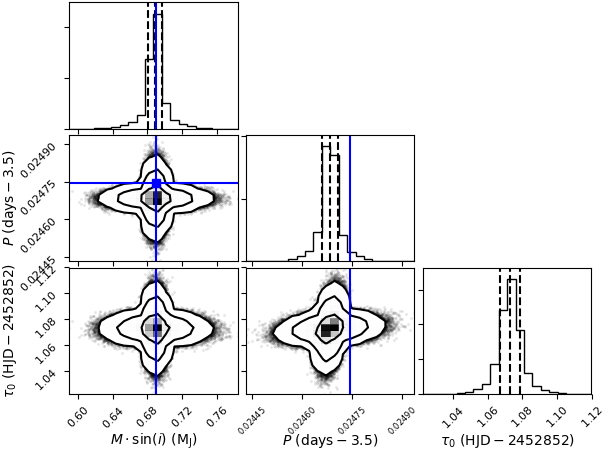
\includegraphics[width=0.75\textwidth]{contours.png}
\vspace{-0.5em}
\caption{The contour plots of the probability distributions and histogram distributions of the parameters. Contours are at 1, 2, and 3$\sigma$. The dashed lines in the histograms represent the mean and a 1-$\sigma$ confidence interval, and the blue lines represent literature values.}
\end{figure}

\vspace{-1em}
\begin{figure}[H]
\centering
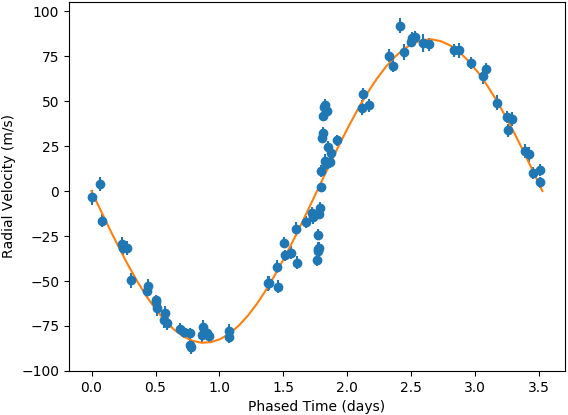
\includegraphics[width=0.75\textwidth]{phasedrv.png}
\vspace{-0.5em}
\caption{The phased RV curve. The literature data points and best-fit solution are shown.}
\end{figure}

\vspace{-1em}
\begin{figure}[H]
\centering
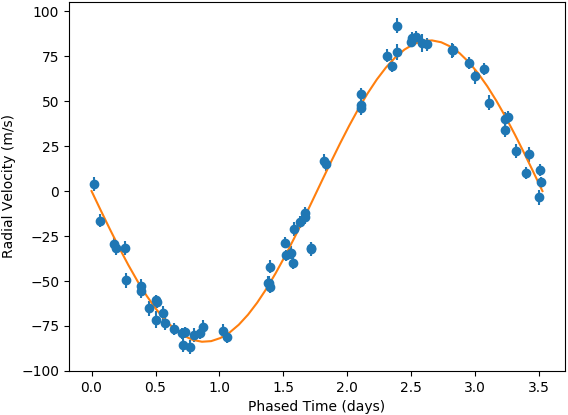
\includegraphics[width=0.75\textwidth]{transitlessrv.png}
\vspace{-0.5em}
\caption{The phased RV curve. The literature data points (excluding the transit epoch) and best-fit solution are shown.}
\end{figure}


\end{document}